% 编辑器使用说明
% 小时物理百科|在线编辑器|latex

\begin{figure}[ht]
\centering
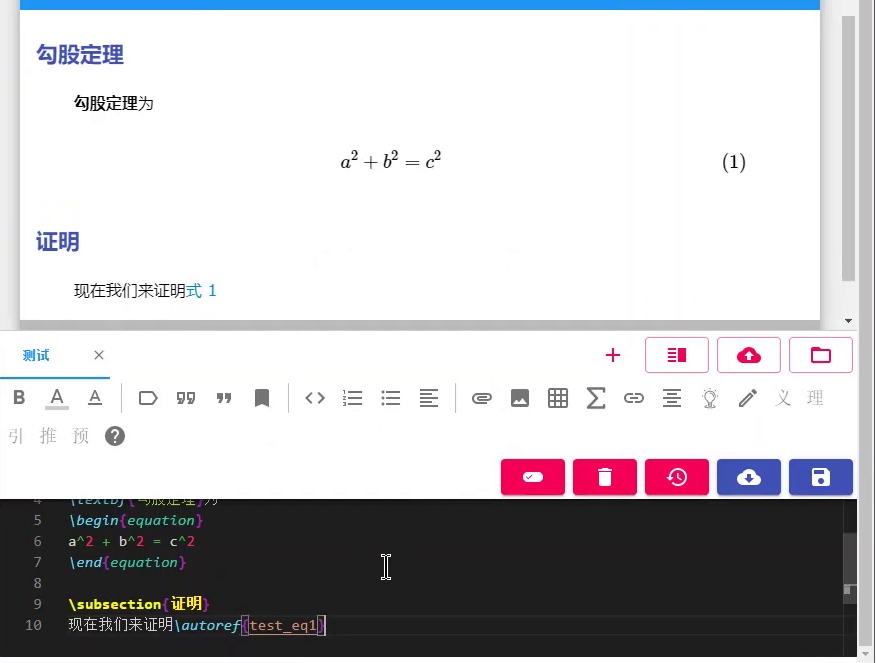
\includegraphics[width=13cm]{./figures/editor_3.png}
\caption{编辑器截图(\href{http://wuli.wiki/apps/editor.gif}{查看 GIF 动画})} \label{editor_fig3}
\end{figure}

\subsection{如果你已经会 LaTeX}
我们必须强调这个编辑器只是在 \href{https://www.mathjax.org/}{MathJax}(仅支持公式) 的基础上做了一个非常简单的拓展, 所以如果你直接把自己的 LaTeX 代码复制进来多半会遇到严重的问题. 我们在 MathJax 的基础上另外实现了一些基本命令如 \verb|\subsection{}|, \verb|\textbf{}|, 常用环境的简单格式以及对他们的引用. 这些功能绝大部分可以在工具栏上找到. 最后, 编辑器只支持百科的模板, 整个百科是一个 \verb|document| 环境, 除了 main.tex 外其他所有 tex 文件都将作为一个 \verb|section| 插入 main.tex 中,不需要手动添加 \verb|\section{}| 命令.

以下大部分不是 LaTeX 的教程而是编辑器的教程, 所以同样建议你大致看一下. 可能大大提高编辑效率的功能有: 引用按钮(自动添加 \verb|\label| 和 \verb|\autoref|), 自动补全和符号替换(在设置按钮里面), 以及各种快捷键.

\subsection{零基础视频教程}
\begin{enumerate}
\item 编辑器使用入门(\href{https://www.bilibili.com/video/av87698355/}{B 站}, \href{https://zhuanlan.zhihu.com/p/105869878}{知乎})
\item 提高编辑效率 (未完成)
\end{enumerate}

\subsection{账号和访问}
\begin{itemize}
\item 若想成为志愿者, 请联系网站管理员申请账号. 如果只是想测试, 可以使用测试网址 \href{http://wuli.wiki/editor-test}{wuli.wiki/editor-test}, 测试账号为 \verb|test1| 到 \verb|test100|, 密码 6 个 \verb|8|. 注意测试账号创建的文件会被定期删除, 可以自行使用下载按钮备份
\item 我们正在测试个人笔记功能, 让每个用户都可以创建自己的百科. 测试网址 \href{http://wuli.wiki/note-test}{wuli.wiki/note-test}. 测试账号和密码同上
\item 推荐使用 Chrome 或者 Chromium 内核的浏览器访问编辑器, 其他浏览器可能存在不兼容问题
\end{itemize}

\subsection{功能简介}

\begin{itemize}
\item 本编辑器使用 LaTeX 语言的一个子集, 一个简单的 LaTeX 介绍见 \href{http://wuli.wiki/online/latxIn.html}{LaTeX 结构简介}
\item 绝大部分命令都可以通过工具栏插入, 所有命令见 “词条示例\upref{Sample}”
\item 进入编辑器初始页面后, 点 “新建词条” 图标(红色加号)可以新建文件, 点 “打开词条” 图标可以编辑已有文件
\item 新建或修改的内容不会立即更新到网站, 而是要审核通过才会发布(有发布权限的用户可以自行发布). 可以在\href{http://wuli.wiki/changed/changed.html}{这里}查看还没有发布的词条以及他们的编辑者
\item 编辑过程中用快捷键 Ctrl+S 可以保存并刷新预览(建议经常刷新, 便于定位错误). 也可以用工具栏的保存图标
\item 我们在模板中用 \verb|\newcommand{}{}| 加入了一些自定义命令, 但不会覆盖原有的 LaTeX 命令. 若希望加入新的自定义命令, 请与管理员协商, 也可以使用下文的 “自动补全” 功能作为代替
\end{itemize}

\subsection{公式}
\begin{itemize}
\item 公式环境支持大部分 LaTeX 命令, 严格来说是所有 \href{https://www.mathjax.org/}{MathJax} 支持的命令\footnote{MathJax 项目用于在网页上显示 LaTeX 公式, \href{https://www.zhihu.com/}{知乎}的公式也使用 MathJax.}
\item 一个简单的公式编辑器见\href{https://www.codecogs.com/latex/eqneditor.php}{这里} (不建议使用, 建议练习手动输入)
\item 一个简单的 TeX/LaTeX 公式入门教程见\href{https://chaoli.club/index.php/211}{超理论坛}
\item 支持部分 \href{http://mirrors.ibiblio.org/CTAN/macros/latex/contrib/physics/physics.pdf}{Physics 宏包}中的命令(见 Sample.tex)
\item 行内公式插入到两个美元符号之间, 如 \verb|$a^2+b^2=c^2$| 显示为 $a^2 + b^2 = c^2$.
\item 独立公式只能用 \verb|equation| 环境(推荐), \verb|align| 环境或者 \verb|gather| 环境. \verb|equation| 环境可以通过工具栏的公式图标插入, 也可以打 \verb|\beq| 然后按 Tab 键或者回车插入, 如
\begin{equation}\label{editor_eq1}
a^2 + b^2 = c^2
\end{equation}
\item 公式中所有常用的和自定义的命令见 “词条示例\upref{Sample}”
\item 为增加代码可读性, 公式中一些命令会显示为对应的符号(如希腊字母, 求和符号, 不等号等), 注意这不会影响源码(复制时得到的也是命令而不是符号). 设置面板(齿轮图标)可以选择关闭该功能
\item 工具栏中的 “内部引用” 按钮可以引用同一页面的公式并生成链接(图片表格等同理), 如\autoref{editor_eq1}. “外部引用” 按钮可以引用其他词条的公式或图表
\end{itemize}

\subsection{用户权限}
每个注册用户默认有编辑词条的权限, 但却不能直接发布词条, 而是需要由发布权限的用户审核后发布. 若一个词条处于 “编辑中” 的状态, 则其他用户无法修改该词条(除非有 “介入编辑” 权限), 只能以只读模式打开. 新建或修改的词条只有通过审核并被发布后才可以被其他用户重新编辑.

\subsection{文件结构}

百科的所有词条是 LaTeX 的一个 \verb|document| 环境, 目录中每个 “部分” 是一个 \verb|\part|, 每个 “章” 是一个 \verb|\chapter|, 每个词条是一个 \verb|\section|, 词条中蓝色的小标题是 \verb|\subsubsection|, 黑色的小标题是 \verb|\subsubsection|. 编辑器打开的一个词条文件就是一个 section 的内容(不需要 \verb|\section| 命令). 用 TeXlive 编译 pdf 的时候所有词条文件都会通过 \verb|\input{xxx.tex}| 插入到主文件 main.tex 中.

网页版的词条目录(\href{http://wuli.wiki/online/}{wuli.wiki/online/})由 main.tex 文件生成, 所以必须修改该文件并发布才能更新目录.

每个词条文件(后缀名为 tex)都有一个独一无二的文件名, 可以将通过将光标停留在编辑器中的 tab 上查看或者通过地址栏的 url 查看.

\begin{figure}[ht]
\centering
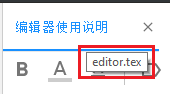
\includegraphics[width=4cm]{./figures/editor_2.png}
\caption{查看词条文件名} \label{editor_fig2}
\end{figure}

每个词条(section) 的 label 与文件名相同, 转换后输出的网页文件(html)也有相同的文件名, 可以在浏览器的地址栏中看到(例如本文的 LaTeX 文件是 \verb|editor.tex|, label 是 \verb|editor|, 转换成网页为 \verb|editor.html|).

\subsection{编辑器说明}
\begin{itemize}
\item 将光标停留在任意按钮上都会出现提示说明按钮的名称. 要新建词条, 点击红色的加号按钮, 根据提示新建即可. 要打开已有词条, 点击最右边的打开, 搜索需要的词条即可
\item 正文中请使用中文标点, 编辑器会自动把空心句号替换为全角实心句号(如果你在使用笔记功能,可以选择在设置中关闭这个功)
\item 编辑器会将有改动的词条每隔 5 分钟备份一次, 可以用 “恢复” 按钮恢复历史版本
\item 编辑器支持各种自动引用(被引用对象没有 label 时会自动插入 label), 工具栏上的\textbf{内部引用}按钮可以引用同一词条的公式, 图表, 例题等环境. \textbf{外部引用}按钮可以引用其他词条的各种环境
\item 如果要在网页预览和 LaTex 代码之间跳转到对应位置, 可以通过搜索关键词实现. 例如在预览窗口复制一段文字, 在编辑窗口搜索就可以跳转到对应内容
\item 任何时候打出反斜杠会自动提示可以自动补全的命令, 用上下键选择, 用 Tab 键或回车确认. 候选词未必是从最左边开始匹配, 例如打 \verb|\bf| 按 tab 就会得到 \verb|\textbf{}|
\item 如果自动补全带括号, 例如 \verb|\frac{}{}|, 补全后光标会自动进入第一个大括号, 再次按 Tab 光标会跳到第二个括号, 再按 Tab 光标会跳到第二个大括号外.
\item 打 \verb|\beq| 按 Tab 会自动出现 \verb|\begin{equation}...\end{equation}|, 其他环境也同理.
\item 用光标选中一串字符后按下加粗按钮, 这串字符会自动插入 \verb|\textbf{}| 中. 同样, 选中字符串后输入 \verb|(| 等括号, 这个字符串会自动插入 \verb|()| 中. 表示行内公式的 \verb|$$| 也支持该操作.
\item 编辑器在生成网页时会将编辑器中的 LaTex 代码转换为通用的 LaTex 代码(网页中右键点击公式获得), 即不需要自定义命令和额外宏包, 可以在任何支持 LaTeX 公式的环境使用(如知乎的公式编辑器).
\item 编辑器支持一键转载到知乎(有少量不兼容, 例如表格和代码), 使用菜单栏的 “导出 Markdown 文件” 按钮, 然后将导出的文件上传到知乎即可. 该功能只能在编辑个人笔记时使用, 未经允许请勿转载百科内容.
\end{itemize}

\subsubsection{快捷键}

\begin{table}[ht]
\centering
\caption{编辑器快捷键}\label{editor_tab1}
\begin{tabular}{|c|c|c|c|}
\hline
保存词条 & \verb|Ctrl| + \verb|S| & 打开词条 & \verb|Ctrl| + \verb|O| \\
\hline
新建词条 & \verb|Ctrl| + \verb|Alt| + \verb|N| & 关闭词条 & \verb|Ctrl| + \verb|Alt| + \verb|W| \\
\hline
显示编辑器选项 & \verb|Ctrl| + \verb|Q| & 跳转到某行 & \verb|Ctrl| + \verb|G| \\
\hline
查找文本 & \verb|Ctrl| + \verb|F| & 替换文本 & \verb|Ctrl| + \verb|H| \\
\hline
向左缩进 & \verb|Ctrl| + \verb|[| & 向右缩进 & \verb|Ctrl| + \verb|]| \\
\hline
增大字号 & \verb|Shift| + \verb|Alt| + \verb|+| & 减小字号 & \verb|Shift| + \verb|Alt| + \verb|-| \\
\hline
关闭不保存 & \verb|Shift| + \verb|点击关闭| &  &  \\
\hline
\end{tabular}
\end{table}

\subsection{编辑器设置}
编辑器中的 “设置” 按钮(齿轮图标)可以添加 “自动补全” 规则. “自动补全” 如上文所描述的, 在输入 LaTeX 命令的过程中, 候选框会显示可以补全的命令, 用上下键选择命令, 然后用 tab 键或回车键补全. 补全规则的格式说明可以点击设置面板中的帮助按钮获得.

设置面板中的也可以添加 “符号替换” 规则. “符号替换” 功能是指, 在 LaTeX 公式中输入一些命令时, 编辑器会自动将其显示为对应的符号, 例如 \verb|\alpha| 显示为 \lstinline|α|, \verb|\sum| 显示为 \lstinline|∑| 等. 这样做是为了增加源码的可读性, 注意这只是一种视觉效果, 不会影响源码本身.
